\documentclass[12pt,oneside]{book}
\usepackage{geometry}                		% See geometry.pdf to learn the layout options. There are lots.
\geometry{a4paper}                   			% ... or a4paper or a5paper or ... 
%\geometry{landscape}                		% Activate for for rotated page geometry
%\usepackage[parfill]{parskip}    		% Activate to begin paragraphs with an empty line rather than an indent
\usepackage{graphicx}				% Use pdf, png, jpg, or epsß with pdflatex; use eps in DVI mode
								% TeX will automatically convert eps --> pdf in pdflatex		
\usepackage{amssymb}

\usepackage[spanish]{babel}			% Permite que partes automáticas del documento aparezcan en castellano.
\usepackage[utf8]{inputenc}			% Permite escribir tildes y otros caracteres directamente en el .tex
\usepackage[T1]{fontenc}				% Asegura que el documento resultante use caracteres de una fuente apropiada.

\usepackage{hyperref}				% Permite poner urls y links dentro del documento

\title{Mi Juego Favorito}
\author{Lenguajes de Programación}
%\date{}							% Activate to display a given date or no date

\begin{document}
\maketitle
\tableofcontents

\chapter{Introducción}
El libro a continuación es creado como una herramienta para el desarrollo de habilidades de edición colaborativa de documentos de texto plano. La herramienta que habilita dicha colaboración, en este taller, es Git pero podría ser reemplazada por otros sistemas de versionamiento.

\chapter{Los Juegos}

\section{Buscaminas}

\begin{figure}[htbp]
\begin{center}
\includegraphics[width=.60\textwidth]{./imagenes/minesweeper.png}
\caption{Buscaminas}
\label{Buscaminas}
\end{center}
\end{figure}
Buscaminas\footnote{\url{http://minesweeperonline.com/}} es uno de los juegos más jugados debido a lo ubicuo de su distribución. Fue incluido en 1992 en la versión de Windows 3.1 y desde entonces lo hemos encontrado presente en todas las versiones de dicho sistema operativo.
En la figura \ref{Buscaminas} puede ver una implementación web del juego.
La premisa del juego es simple: Limpiar el campo de juego sin hacer explotar ninguna de las minas que se encuentran en la cuadrícula.

\subsubsection{¿Por qué es uno de mis juegos favoritos?}
\begin{itemize}
\item[Javier Tibau] Las reglas del juego son sencillas y fáciles de entender. A pesar de esto, el juego no es atractivo para todo el mundo, creo que es un gusto adquirido. Las reglas me fueron presentadas por mi papá, quien en su máquina de trabajo con Windows 3.11 era uno de los pocos juegos ``divertidos'' que tenía. Para mi, el gran interés del juego es que destaca (o esconde) la resolución de problemas con fondo algebraico. En cierto momento del juego, y para el jugador que ha estudiado álgebra lineal, el reventar una casilla se torna similar a descifrar un sistema de ecuaciones con varias incógnitas. Los sistemas sencillos son bien definidos y tienen 2, 3 o hasta 4 incógnitas, mientras los más complejos pueden inclusive tener múltiples soluciones.
\end{itemize}

\section{Dota 2}

\begin{figure}[htbp]
\begin{center}
\includegraphics[width=.60\textwidth]{./imagenes/dota2.jpg}
\caption{Dota 2}
\label{Dota 2}
\end{center}
\end{figure}
Dota 2 \footnote{\url{http://dota2.com/}} es un juego creado por Valve basado en el popular mod de Warcraft 3, Defense of the Ancients. Es un juego de estrategia en equipo para ser jugado con equipos de 5 personas cada uno.
Dota 2 combina elementos de estrategia en tiempo real con perspectiva "en tercera persona", incorporando a todo ello un sistema de nivelación y jugabilidad de diversos juegos de rol como Diablo. Los jugadores asumen el papel de una unidad clasificado como un "héroe", que puede subir de nivel hasta un máximo de 25. La configuración básica de Dota 2 consiste en dos ciudades de distinta forma, cada una cuenta con una fortaleza de defensa conocida como "ancestro", situadas en los extremos opuestos de un mapa equilibrado de manera uniforme. Entre ellas hay varias regiones de conexión identificado como "caminos", que son atravesados por unidades enemigas, al tiempo que luchan contra poderosas torres defensivas a lo largo del camino. Los jugadores se dividen entre dos equipos, cada uno con hasta cinco jugadores, para competir como los principales defensores de cada Fortaleza de los Ancestros.

\subsubsection{¿Por qué es uno de mis juegos favoritos?}
\begin{itemize}
\item[Victor Cedeño] Este es un juego que requiere de comunicación y cooperación entre 5 personas para poder lograr el objetivo de vencer al otro equipo. Es muy dificil jugar solo sin la ayuda de tus compañeros. El juego tiene una gran selección de más de 100 heroes para elegir, esto quiere decir que cada partida es diferente ya que las combinaciones posibles de los equipos son innumerables. Es un juego que fomenta el trabajo en equipo y las decisiones correctas.
\end{itemize}

\include{juegos/Zelda}
\section{Temple Run}

\begin{figure}[htbp]
\begin{center}

\includegraphics[width=.35\textwidth]{./imagenes/templerun.png}
\caption{Temple Run}
\label{Temple Run}
\end{center}
\end{figure}
En todas las películas de aventuras hay una escena donde el héroe finalmente pone sus manos en el tesoro, pero entonces tiene que atravesar una gran cantidad de trampas para salir vivo. Temple Run\footnote{\url{https://itunes.apple.com/es/app/temple-run/id420009108?mt=8}} es esa escena. Y es asombrosa. Es una de las aplicaciones mas solicitadas tanto en la App Store, como en Google Play por su atractiva interfaz, y por lo divertido de sus niveles. Siéntete como un auténtico buscador de tesoros, y diviértete escapando de los villanos, saltando rampas, esquivando objetos y consiguiendo monedas y poderes.

\subsubsection{¿Por qué es uno de mis juegos favoritos?}
\begin{itemize}
\item[Charlie Medina] Es un juego simple, pero que puede proporcionar horas de entretenimiento. Fue uno de los primeros juegos que descargué cuando consegui un iPhone, y recuerdo que pasé horas jugandolo hasta haber superado los primeros niveles. Lo interesante del juego, es que compites contra ti mismo, ya que lo único que buscas es superar tu propio récord, tratando de llegar cada vez mas lejos, consiguiendo mas monedas (que luego te sirven para comprar objetos) y desbloqueando poderes que te ayudarán a evadir las trampas o que te salvarán de alguna caída, y te permitirán llegar cada vez más lejos. Como el juego no tiene un final, puedes pasar el tiempo que quieras tratando de superarte, y a medidad que llegas mas lejos, se dificulta ya que la velocidad incrementa y tienes que volverte un experto hábil para esquivar objetos a grandes velocidad. Sin duda, recomendado para todos aquellos con smartphones y con bastante tiempo libre.
\end{itemize}
\section{Resident Evil}

\begin{figure}[htbp]
\begin{center}
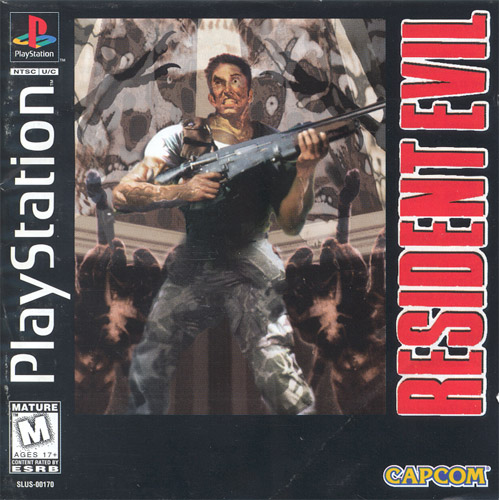
\includegraphics[width=.35\textwidth]{./imagenes/resident_evil1.jpg}
\caption{Resident Evil}
\label{Resident Evil}
\end{center}
\end{figure}
Una extraña ola de asesinatos empiezan a ocurrir en las montañas Arklay a las afueras de Racoon City.  Es entonces que la noche del 24 de julio de 1998 el departamento de policia de Racoon City envia al equipo Bravo del gurpo especial S.T.A.R.S. (Special Tactics And Rescue Service) a investigar. Al poco tiempo se pierde el contacto con el equipo Bravo y se envia al equipo Alpha a continuar la investigacion y encontrar al equipo Bravo. Al llegar son atacados por una especie de perros zombies y son obligados a refugiarse en una mansion cercana. Es Aqui Donde comienza la pesadilla de los S.T.A.R.S. por sobrevivir ya que la mansion es un centro secreto de desarrollo de armas biologicas, y los miembros de S.T.A.R.S. han sido engañados para probar una nueva arma denominada Virus-T la cual es capaz de reviir el tejido muerto a nivel celular. En Resident Evil\footnote{\url{http://www.residentevilcenter.net/residentevil.html}} entramos en la piel de los miembros del equipo Alpha de S.T.A.R.S. Chris Redfield o Jill Valentine los cuales se enfrentaran a monstruos creados con el virus-T tales como zombies y demas criaturas; con municion limitada y su sentido de supervivencia.

\subsubsection{¿Por qué es uno de mis juegos favoritos?}
\begin{itemize}
\item[Joseph Gallardo] Es un juego del genero Survival Horror el cual se caracteriza por su camara estatica, y la escasa municion la cual habra que utilizarla sabiamente, ya que habra ocasiones en las que sera mejor huir antes que pelear. La historia del juego es exelente, los puzzles son un verdadero reto y las desiciones que tomes durante el juego afectan al final de la historia. Es uno de mis videojuegos favoritos ya que lo considero como un verdadero reto para superar.
\end{itemize}
\section{Gatos Gemelos}

\begin{figure}[htbp]
\begin{center}
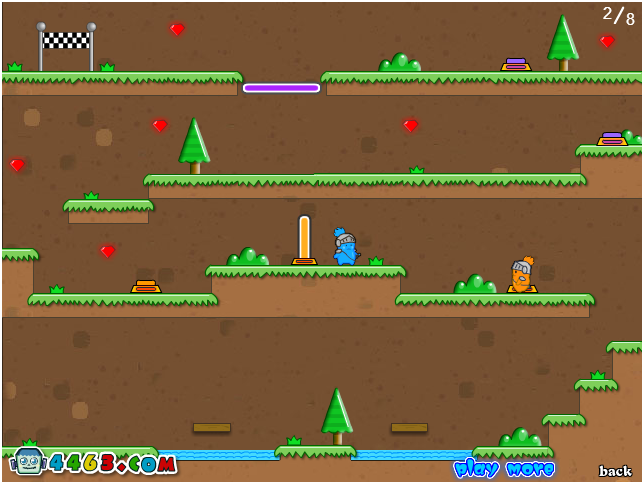
\includegraphics[width=.60\textwidth]{./imagenes/gatos.png}
\caption{Gatos Gemelos}
\label{Gatos Gemelos}
\end{center}
\end{figure}
Gatos Gemelos \footnote{\url{http://ar.yayoye.com/twin-cat-online-game/22643/}} es un Juego en el que se deben mover a los personajes por la pantalla, como su nombre mismo lo dice son unos gatos gemelos, con los que iremos tratando de recoger diamantes y de lograr que interactúen entre ellos para superar los obstáculos.

\subsubsection{¿Por qué es uno de mis juegos favoritos?}
\begin{itemize}
\item[Tania Sánchez] En realidad no soy de esas personas que se vician con los juegos pero me llaman mucho la atención el tipo de juego que estimula el aprendizaje, me parece que este juego lo hace, ya que es un juego que se realiza en pareja en el que enseña el trabajo en equipo, a medida que avanzan los niveles va aumentando la dificultad del mismo, poniendo al usuario cada vez a pensar más en como vencer los obstaculos tomando en cuenta que un jugador debe ir a la par con el otro e irlo ayudando para juntos llegar a la meta, la dificultad del juego aparte de resolver como se debe avanzar, está en no olvidarse del compañero ya que aunque llegue uno de los dos solo a la meta no implicará que se pasará al siguiente nivel sino que deben llegar los dos juntos. 
\\
\\
Éste es un juego orientado más para niños pequeños para estimular el desarrollo intelectual y enseñarles el trabajo en equipo =).
\end{itemize}
\section{Twisted Metal: }

\begin{figure}[htbp]
\begin{center}
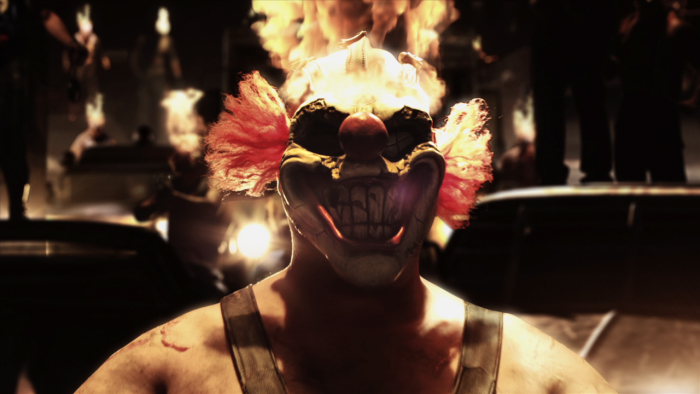
\includegraphics[width=.60\textwidth]{./imagenes/twistedmetal.jpg}
\caption{Twisted Metal}
\end{center}
\end{figure}

Twisted Metal es la primera entrega de la serie Twisted Metal. La historia del juego está centrada en el titular de la competencia en la que varios conductores de vehículos modificados deben destruir los otros vehículos en un intento por ser el último vivo. El ganador se reúne con el organizador de la competición, un misterioso hombre llamado Calypso, que otorgará al ganador un único deseo, independientemente de su precio, tamaño, o incluso de la realidad.
Twisted Metal recibió críticas dispares de la prensa especializada, pero el juego fue un éxito comercial, vendiendo más de 1.800.000 copias en los Estados Unidos.
\subsubsection{¿Por qué es uno de mis juegos favoritos?}
\begin{itemize}
\item[Juan Romero ] Twisted Metal es una de mis franquicias de juegos favoritos. He sido  fan desde hace mucho tiempo y comenzé a jugar la serie con Twisted Metal 3 para la consola de PlayStation 1 . Lo que me gustó de la experiencia fue que se combinan de forma única los juegos de conducción con los de  shooter en primera persona. Matar a los oponentes y ver como volaban en mil pedasos era lo que mas me divertia, ademas el hecho de que habia que tener buenas habilidades para manejar un vehículo,matar y estar pendiente de eludir los ataques de los demas contrincantes.
\end{itemize}
\section{Mortal Kombat Armageddon}

\begin{figure}[htbp]
\begin{center}
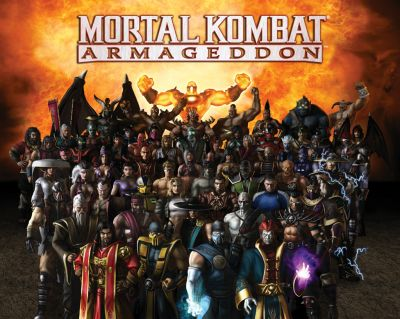
\includegraphics[width=.60\textwidth]{./imagenes/MortalK.jpg}
\caption{Mortal Kombat Armageddon}
\label{Mortal Kombat Armageddon}
\end{center}
\end{figure}

Mortal Kombat: Armageddon \footnote{\url{http://www.mortalkombat.net/armageddon/}} es un videojuego de la saga Mortal Kombat desarrollada por Midway Games. Este juego es una continuación directa de Mortal Kombat: Deception. El juego distribuyo más de 2 millones de copias por todo el mundo.
Las plataformas designadas para este juego son PlayStation 2 y Xbox en el 2006 y Wii en el 2007.

\subsubsection{¿Por qué es uno de mis juegos favoritos?}
\begin{itemize}
\item[Joao Sanga] Me gusta mucho por los gráficos, el modo de pelea y la historia. Las peleas en Mortal Kombat siempre conservarán su puntito gore (sangriento): sin él, nada diferenciaría a la saga de otros tantos juegos de lucha.
Aprendiendo de la experiencia en títulos pasados, MK Armageddon ha suavizado los controles, y ha ordenado todos los elementos en un sencillo menú. Pero la mecánica del juego sigue siendo la misma: cada luchador tiene dos métodos de combate –una técnica cuerpo a cuerpo, y lucha con arma-, junto con los clásicos combos aéreos, encadenados, llaves y contras. Quienes busquen un título de machaque fácil pulsando botones a toda velocidad, lo tienen complicado de nuevo: en Mortal Kombat los combates no lo parecen, SON lentos, ni de lejos tan vertiginosos como en cualquier juego de lucha de Namco. Los kombatientes se mueven en ocasiones como marionetas que responden mecánicamente a nuestras teclas.
En conclusión, Mortal Kombat Armageddon es uno de los mejores creados de la saga de Mortal Kombat.
\end{itemize}
\section{World Of Warcraft}

\begin{figure}[htbp]
\begin{center}
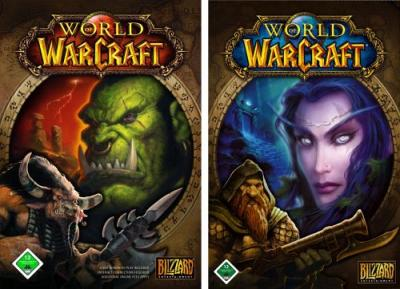
\includegraphics[width=.60\textwidth]{./imagenes/wowclasic.jpg}
\caption{World Of Warcraft}
\label{World Of Warcraft}
\end{center}
\end{figure}

World of Warcratf es uno de los mejores juegos online que existe a nivel mundial, la primera version de este juego fue lanzada en el año 2004 siendo denominada como Clásica, pocos años despues se fueron añadiendo nuevas expansiones, cada una de estas implementaron nuevos desafios y mejoras, haciendo que la gente quedara con la ganas de obtenerlo y jugarlo.

Una de las principales atracciones que obtuvo el juego fue la manera de implementar una gran cantidad de razas y clases, dentro de las que podemos definir las siguientes:

\large{Razas}
\begin{itemize}
\item Humano  \item Enano  \item Gnomo  \item Elfo de la noche 
\item Orco  \item No-muerto  \item Tauren  \item Trol
\end{itemize}

\large{Clases}
\begin{itemize}
\item Paladin  \item Chaman  \item Druida  \item Guerrero
\item Picaro  \item Sacerdote  \item Cazador  \item Brujo  \item Mago
\end{itemize}
\newpage
\begin{figure}[htbp]
\begin{center}
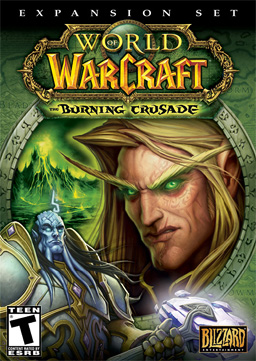
\includegraphics[width=.60\textwidth]{./imagenes/wowtbc.jpg}
\caption{World Of Warcraft: The Burning Crusade}
\label{World Of Warcraft: The Burning Crusade}
\end{center}
\end{figure}
La primera expansión lanzada en el año 2007, en el cual se implementaron 2 nuevas razas, una nueva ciudad,  un nuevo tipo de Campo de Batalla y un sistema de juego llamado Arenas. Ademas de que los Pjs podian alcanzan un nivel máximo de 70.

\begin{itemize}
\item Dranei
\item Elfo de sangre
\end{itemize}

\newpage
\begin{figure}[htbp]
\begin{center}
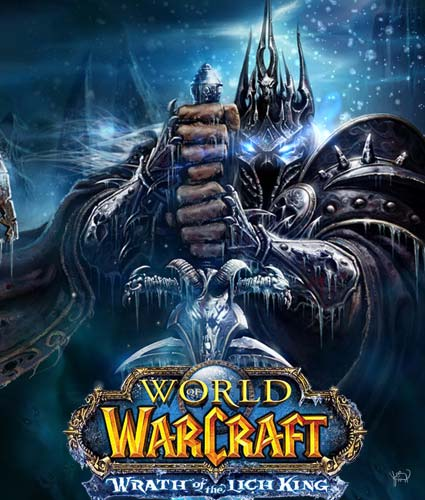
\includegraphics[width=.60\textwidth]{./imagenes/WOW.jpg}
\caption{World Of Warcraft: Wrath of the Lich King}
\label{World Of Warcraft: Wrath of the Lich King}
\end{center}
\end{figure}
Segunda expansión lanzada en el año 2008, dentro de esta la implementacion fue un nuevo continente Rasganorte, además de que se cuenta con llevar a los Pjs a un nivel de 80 y la implemtación de una nueva clase. Nuevas estancias de Mazmorras y Bandas fueron incluidas dentro de esta expansión por causa del nuevo continente.

\begin{itemize}
\item Caballero de la Muerte
\end{itemize}

\newpage
\begin{figure}[htbp]
\begin{center}
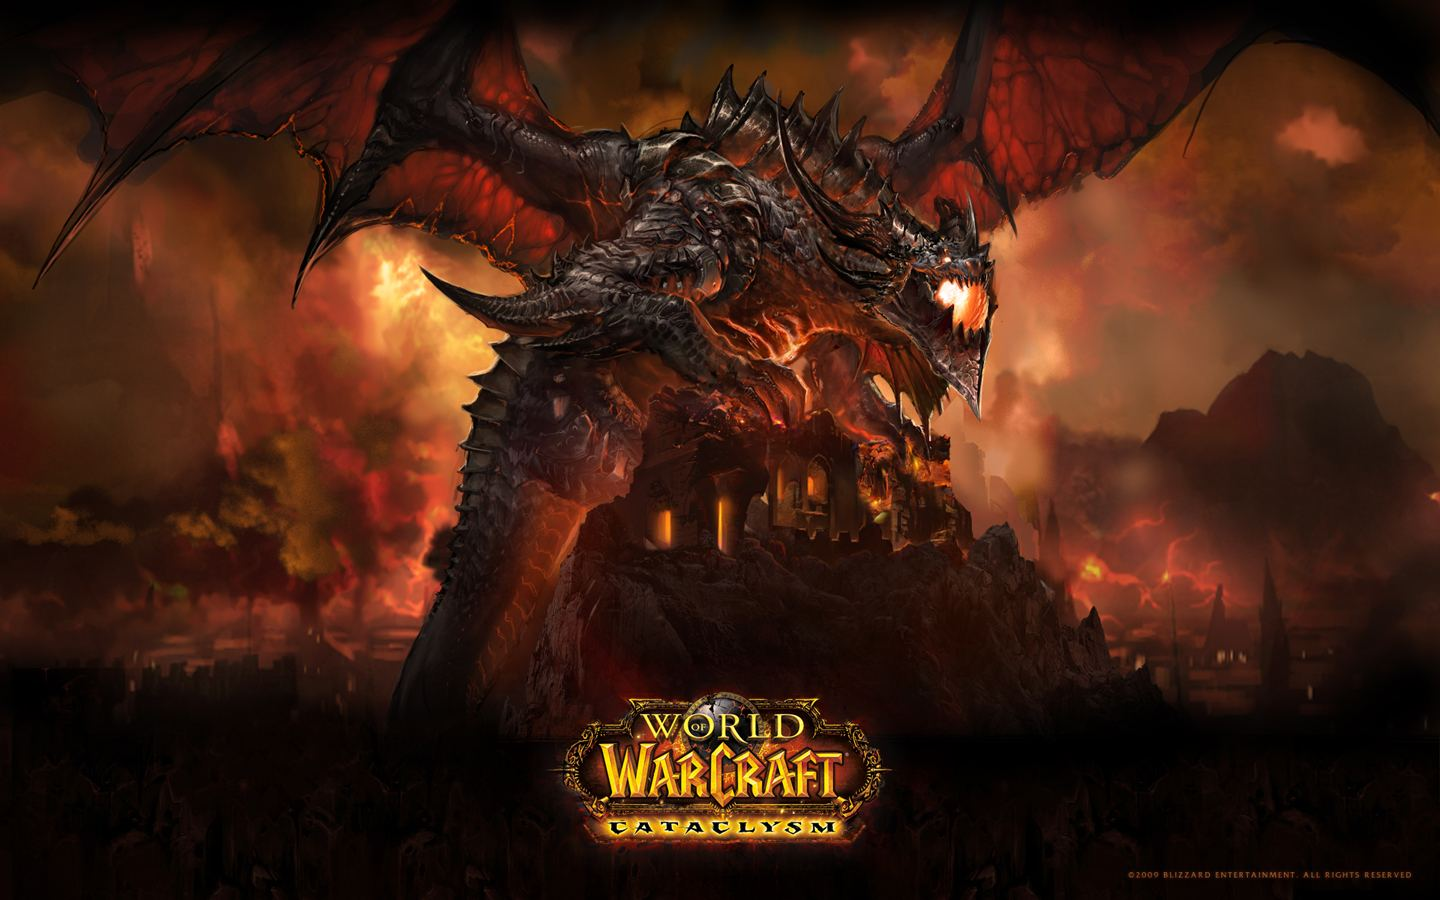
\includegraphics[width=.60\textwidth]{./imagenes/wowcataclysm.jpg}
\caption{World Of Warcraft: Cataclysm}
\label{World Of Warcraft: Cataclysm}
\end{center}
\end{figure}

Tercera expansión lanzada en el año 2010, la implementación para esta expansión fueron 1 nueva raza para cada facción, ademas de una nueva profesión secundaria y el nivel alcanza el 85. Las ciudades principales tanto de la Alianza como la Horda sufrieron cambios con respecto a sus aspectos.

\begin{itemize}
\item Huargen
\item Goblin

\item Arqueologia
\end{itemize}

\newpage
\begin{figure}[htbp]
\begin{center}
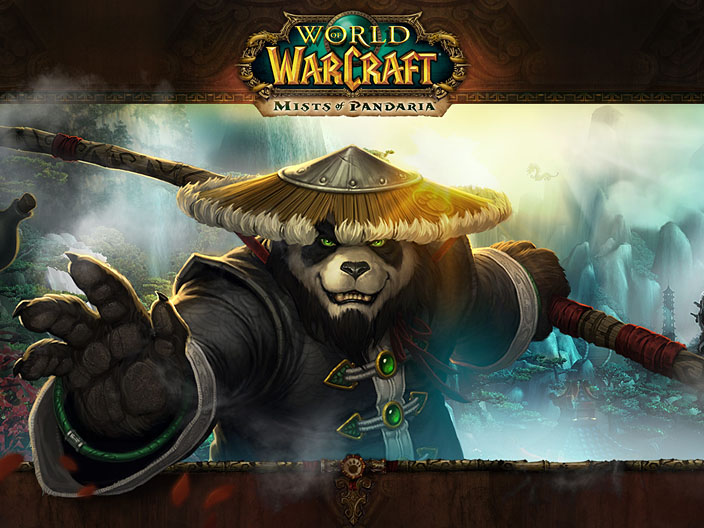
\includegraphics[width=.60\textwidth]{./imagenes/wowpandaren.jpg}
\caption{World Of Warcraft: Mists of Pandaria}
\label{World Of Warcraft: Mists of Pandaria}
\end{center}
\end{figure}
Cuarta y última expansión conocida actualmente, se inclyó una nueva raza junto con una nueva clase para las facciones, ademas de un nuevo continente, se cuenta con la implementación de nuevas mazmorras y desafios, en esta última expansión el limite de nivel es 90.

\begin{itemize}
\item Pandaren
\item Monje
\end{itemize}

Sufriendo muchos cambios durante cada expansión el juego tiende a convertirse en adictivo, a pesar de que ya no es el juego mas jugado en el mundo sigue estando con su record mundial.

\subsubsection{¿Por qué es uno de mis juegos favoritos?}
\begin{itemize}
\item[Marlon Loayza] La razón por la que es mi juego favorito se debe a la trama he historia que posee cada una de las razas dentro del juego, creando sus alianzas y combatiendo por el poder, la manera en la que te permite crear estrategias para la batalla es una de las razones mas fuertes de seguirlo jugando, ya que no luchas simplemente contra una maquina, cada jugador es una mente diferente y aplican diferentes tecnicas para combatir, haciendo que obtengas muchos desafios y te permite crear tus formas de jugar, la interacción virtual que haces con los demas jugadores hace que el juego sea mas entretenido ya que en ciertos casos estamos obligados a trabajar en grupos, lo que nos lleva a tener una buena comunicación. 
\end{itemize}

\section{The conquers II}

\begin{figure}[htbp]
\begin{center}
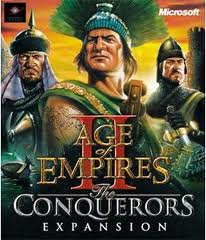
\includegraphics[width=.37\textwidth]{./imagenes/conquers.jpg}
\caption{The conquers II}
\label{The conquers II}
\end{center}
\end{figure}
The conquers II  es un videojuego de estrategia en tiempo real para computadoras personales, desarrollado por Ensemble Studios y publicado por Microsoft Games para las plataformas Microsoft Windows y Apple Macintosh. El título expande al videojuego Age of Empires II: The Age of Kings y fue lanzado a mediados del año 2000.
Mantiene el mismo guion en su desarrollo tanto económico como militar, no obstante introduce algunas mejoras en la IA de algunas unidades que ayudan a tener más tiempo para plantear una estrategia, introduciendo civilizaciones americanas (Mayas y Aztecas), además de algunas otras civilizaciones (Españoles, Hunos y Coreanos), más modos de juego y nuevos mapas.

\subsubsection{¿Por qué es uno de mis juegos favoritos?}
\begin{itemize}
\item[Keyla Figueroa] Este juego se basa en armar estrategias, tanto de ataques como de defensa. 
El juego comienza con cierta cantidad de aldeanos, a estos se les asigna diferentes tareas como recolectar madera, alimentos, oro y roca. En base a lo que ellos recolectan, se construyen casas, establos, cuarteles, etc, hasta llegar a armar un imperio con tus propias reglas. El objetivo principal de este juego es derrotar a todos los imperios existentes, quedando así como el único imperio conquistador.
Lo que más me gusta de este juego es que estimula el cerebro al momento de tomar decisiones, a liderar frente a diversas situaciones, y a conocer más sobre las culturas occidentales y orientales del mundo. 
\end{itemize}
\section{Bioshock}

\begin{figure}[htbp]
\begin{center}
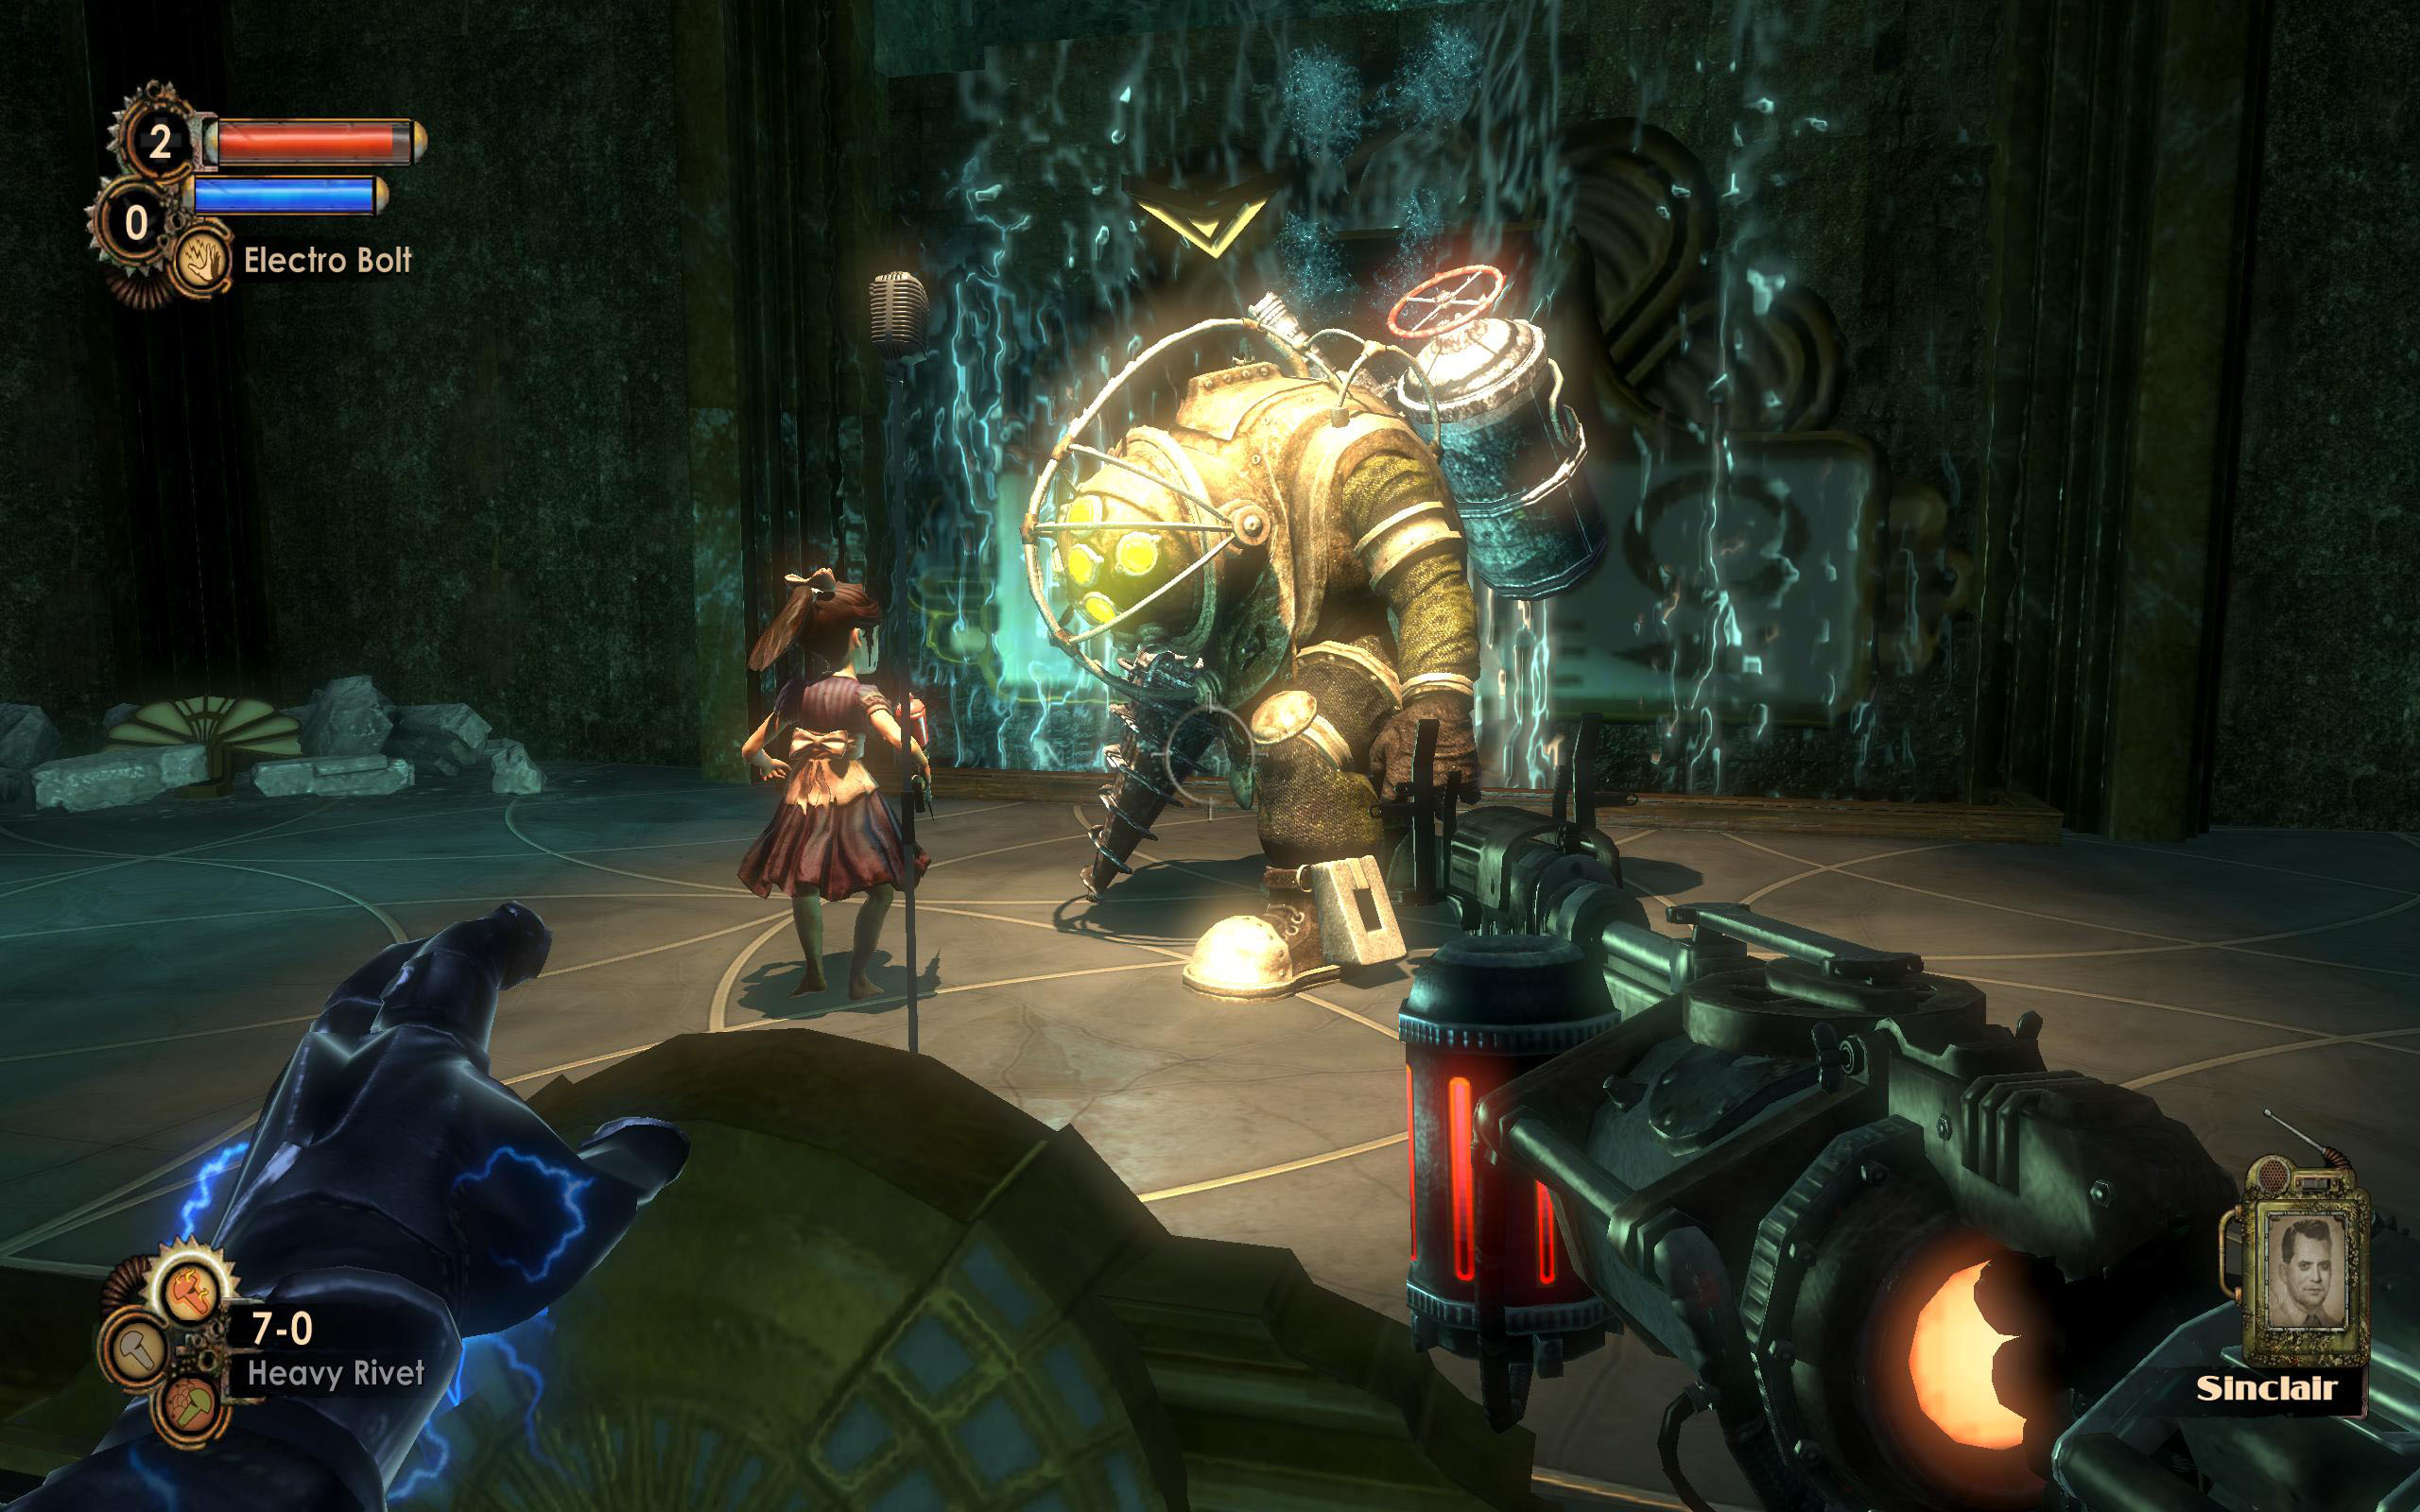
\includegraphics[width=.60\textwidth]{./imagenes/bioshock.jpg}
\caption{Bioshock}
\label{Bioshock}
\end{center}
\end{figure}
Bioshock\footnote{\url{http://http://www.bioshockgame.com/}} es un juego de disparos en primera persona desarrollado por Irrational Games.

El protagonista, luego de caer al océano debido un accidente aéreo, llega a una ciudad submarina llamada Rapture. Construida por un magnate de negocios con el objetivo de llegar a ser una utopía aislada, regida únicamente por los principios filosóficos libertarios seguidos por el magnate. ``Ni Dios, ni reyes. Solo el hombre'' se puede leer en un gran letrero a la entrada de Rapture.

Sin embargo, al llegar, ya es una ciudad fantasma cayéndose a pedazos, con las pocas personas que quedan completamente locas, y la mayoría siempre en busca de una dosis de una droga energética desarrollada en Rapture.

El jugador se debe abrir camino utilizando armas e inyecciones para alterar su genética, además de tener que hackear algunos dispositivos para poder obtener comida y municiones.

\subsubsection{¿Por qué es uno de mis juegos favoritos?}
\begin{itemize}
\item[Ramón Carrillo] No solo es un juego de acción, el elemento más destacable es la historia y la profundidad de los personajes, se discuten aspectos morales, religiosos, políticos y filosóficos. La intriga está presente todo el tiempo: ¿cómo se construyó la ciudad?, ¿cuál fue la motivación?, ¿qué hizo que fracasara?, ¿qué pasó con sus promotores?. Y finalmente el aspecto retrofuturista de Rapture y los sonidos que provienen ya sea de un robot o de otro esquizofrénico habitante lo convierten en un juego que atrapan tu concentración totalmente.
\end{itemize}

\section{Need For Speed Hot Pursuit}

\begin{figure}[htbp]
\begin{center}
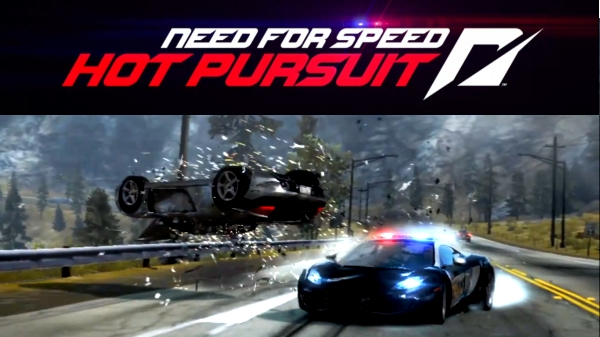
\includegraphics[width=.60\textwidth]{./imagenes/NeedForSpeedHotPursuit.jpg}
\caption{Need For Speed Hot Pursuit}
\label{Need For Speed Hot Pursuit}
\end{center}
\end{figure}

Need For Speed Hot Pursuit\footnote{\url{http://www.needforspeed.com/es_ES/hot-pursuit}}es el nombre de la decimocuarta entrega de la saga Need for Speed. Es un juego de carreras de 2010 desarrollado por Criterion Games y publicado por Electronic Arts para PlayStation 3, Xbox 360, Microsoft Windows, Wii y iPhone.6 7 También hay una versión para Wii, desarrollada por Exient. El juego ha sido descrito como una "revolucionaria" adición de la saga Need for Speed y fue lanzado enNorteamérica el 16 de noviembre de 2010, y en Europa el 18 de noviembre.

El juego está inspirado en Need for Speed: Hot Pursuit original, basado a su vez en las persecuciones de alta velocidad con autos exóticos. Como se ha visto en juegos anteriores, en Hot Pursuit se tiene la oportunidad de ser un policía o un piloto huyendo de la justicia. Hot Pursuit se centra en un lugar ficticio llamado Seacrest County, lugar muy abierto que permite al jugador correr durante varios kilómetros.

\subsubsection{¿Por qué es uno de mis juegos favoritos?}
\begin{itemize}
\item[Esteban Muñoz]Este consiste en que el jugador tiene que ganar la carrera escapando de la      policía, o jugar como policía e intentar dar caza y arrestar a los pilotos que infringieran los límites de velocidad. Muchos de los coches y circuitos no están disponibles al comenzar el juego. El objetivo es desbloquearlos al ganar carreras.El juego disponía de coches exóticos como el Lamborghini Diablo SV, Mercedes-Benz CLK GTR o el Jaguar XJR-15,coches especiales (el phanton y el titan) cuyas características son de estabilidad y velocidad extrema,los cuales aparecen en el juego por medio de claves especiales escritas en el user name y un coche inventado por los creadores (siendo este el de mejor características) llamado "El Niño" y en el modo hot pursuit tiene como extra un helicóptero de policía. Además incluye pistas como una en la que se pasa debajo de un túnel de cristal, en una especie de lago o una ciudad. Pasando por cañones, por zonas rurales, e inclusive carreteras urbanas. Otra característica era que el trazado podía ser de noche o de día y con lluvia o nieve.
\end{itemize}

\section{ Hitman Código 47}

\begin{figure}[htbp]
\begin{center}
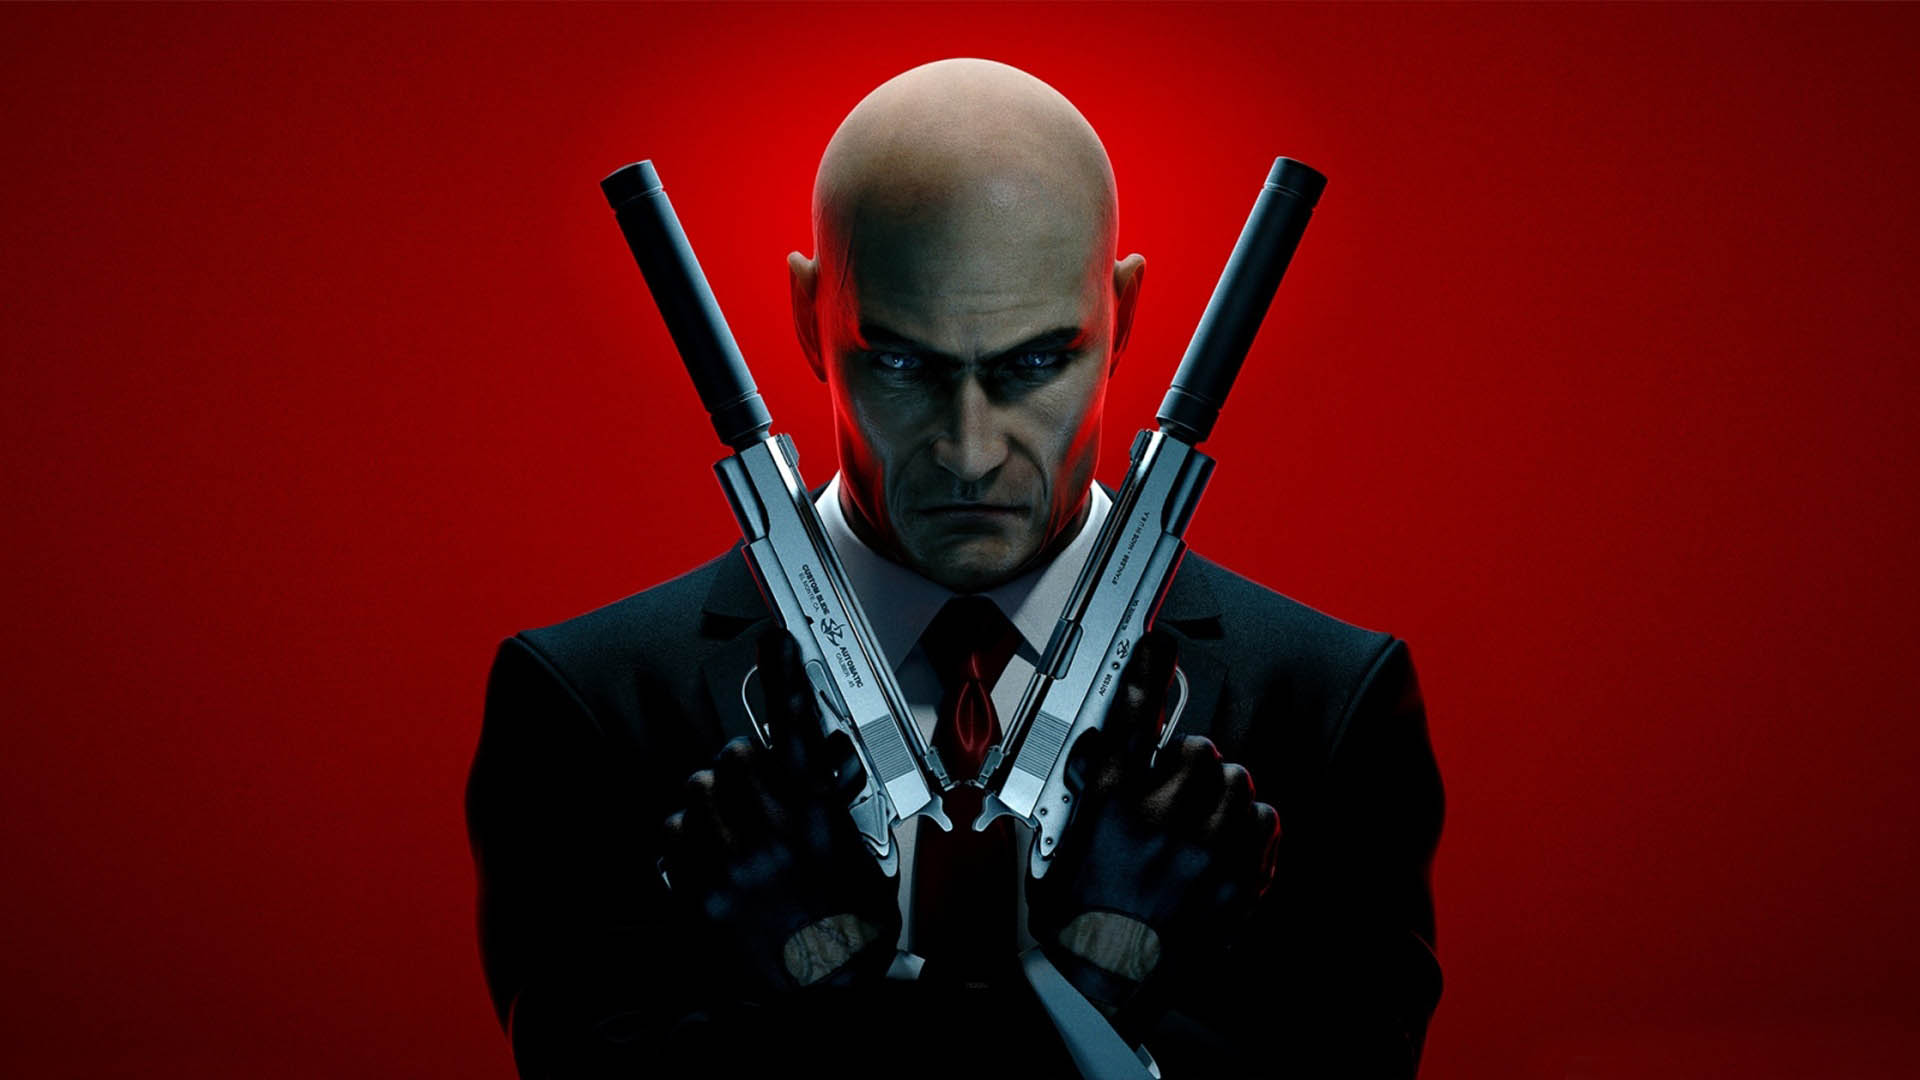
\includegraphics[width=.60\textwidth]{./imagenes/hitman.jpg}
\caption{ Hitman Código 47}
\label{ Hitman Código 47}
\end{center}
\end{figure}
Castlevania\footnote{\url{http://www.guiamania.com/page.php?v=011518/}} es un videojuego de disparos en tercera persona creado por la compañía IO Interactive y publicado por Eidos Interactive en 2000. Es el primer videojuego de la saga de Hitman. Como en todos los juegos de la saga, el personaje principal es el Agente 47, un sicario que trabaja para la ICA (International Contract Agency, Agencia Internacional de Contratos), se divide en varias historias principales, cada una con sus niveles. Antes de cada nivel, la Agencia le da la oportunidad al jugador de seleccionar algunas de las armas y el equipo que va a llevar consigo a la misión, según el dinero que haya obtenido en las anteriores fases. Una vez estudiados los informes de cada objetivo, así como las fotos o los mapas que le puedan ser proporcionados, el jugador inicia la misión. El jugador maneja al propio 47, asesino a sueldo muy habilidoso y sigiloso. En esta, como en todas las entregas de la saga, se castigan los asesinatos de civiles, ya sean peatones, meseros u otros, y lo hace descontando dinero al final de la misión, pudiendo ser considerada fallida si el balance económico es desfavorable para el protagonista. Es por esto que no es un juego en el que la táctica principal sea el enfrentamiento directo con el oponente y matar a diestra y siniestra. Es el engaño y el sigilo la principal arma con que el jugador cuenta. Desde no cargar armas a la vista u obtener información de los personajes con que interactúa hasta otras más sofisticadas, como matar silenciosamente (con una cuerda de piano o un cuchillo) esperando el momento de encontrarse a solas con el objetivo o disfrazarse con las ropas de alguna víctima, son ejemplos de las características del juego. Añadido a eliminar a los objetivos de cada misión, 47 deberá realizar otras tareas secundarias, como esconder cadáveres, desactivar bombas, o liberar inocentes; algunos de ellos le darán información valiosa para el transcurso de la misión..

\subsubsection{¿Por qué es uno de mis juegos favoritos?}
\begin{itemize}
\item[Juan Mite]  Fue la primera parte de una serie de juegos de este asesino a sueldo. Las graficas eran muy buenas para la epoca en que se lanzo debe ser por eso que me impactó.  La trama a simple vista puede ser algo simple (un simple asesino) pero las misiones no son triviales excepto las primeras.  A medida que completes misiones el juego se pondrá más difícil puesto que los blacos tienes mas seguridades varían entre: Diputados, Narcotraficantes, Presidentes, Senadores, Jefes de carteles. 
\end{itemize}

\section{Deus Ex: Human Revolution}

\begin{figure}[htbp]
\begin{center}
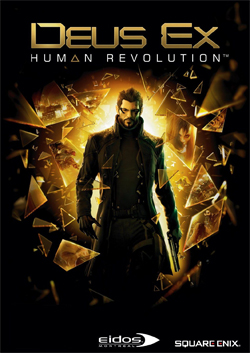
\includegraphics[width=.60\textwidth]{./imagenes/deusex.jpg}
\caption{Deus Ex: Human Revolution}
\label{Deus Ex: Human Revolution}
\end{center}
\end{figure}
Deus Ex: Human Revolution\footnote{\url{http://www.deusex.com/}}  es la precuela del aclamado "Deus Ex", lanzada en Agosto del 2011 por Eidos Montreal. Es un juego que se lleva a cabo en un futuro no muy distante, donde las aumentaciones (implantes físicos) son cosas del día a día, y que dan poder a quién las tenga.
En medio de todo esto se encuentra el protagonista, Adam Jensen, el cual se ve inmerso en un complot que abarca el destino de la humanidad.

\subsubsection{¿Por qué es uno de mis juegos favoritos?}
\begin{itemize}
\item[Luis Vasquez] Como un fanático de la serie, me fué natural comprar este juego en el día de lanzamiento, y no fui decepcionado. A parte de la gran trama que este juego ofrece , la cual no le pide favores a la del original, este logra modernizar todos los aspectos de jugabilidad
de  Deus Ex, asi como ofrecer al jugador varias opciones de juego, uno puede elegir entre sigilosamente infiltrarse en la base enemiga sin ser visto, o simplemente asesinar a sangre fría a cualquiera que se te cruze en tu camino.
\end{itemize}

\section{Assassin's Creed: Revelations}

\begin{figure}[htbp]
\begin{center}
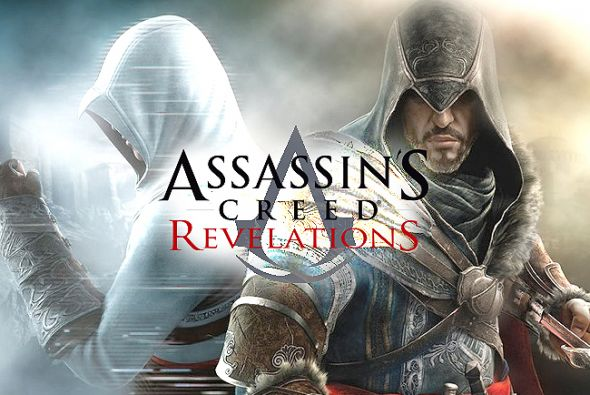
\includegraphics[width=.60\textwidth]{./imagenes/Revelations.jpg}
\caption{Assassin's Creed: Revelations}
\label{Assassin's Creed: Revelations}
\end{center}
\end{figure}
Assassin's Creed: Revelations\footnote{\url{http://assassinscreed.ubi.com/ac3/es-es/games/assassins-creed-revelations/index.aspx}} El juego comienza varios años después de Assassin's Creed: Brotherhood en el papel de Ezio, ya varios días con Lucy muerta, Desmond Miles en coma y Rebecca, Shaun y el misterioso William M. tratando de reanimar a Desmond, mediante el Animus. Desmond para tratar de salvarse, explorará los últimos días de las vidas de Altaïr Ibn-La'Ahad y Ezio Auditore, para crear un nexo de sincronización. 


\subsubsection{¿Por qué es uno de mis juegos favoritos?}
\begin{itemize}
\item[Luis Caviedes]Assassin’s Creed: Revelations hace gala a su nombre, ya que su historia une cabos sueltos de la franquicia y, sobre todo, sirve de nexo entre Ezio Auditore, Altaïr ibn La-Ahad y Desmond Miles, justamente los tres personajes jugables de este juego. La excelente jugabilidad es una marca de fábrica de la saga Assassin’s Creed. Revelations no es la excepción, otorgándonos un control de personaje soberbio. La ambientación de Constantinopla es sobrecogedora. Los detalles de los edificios, las mezquitas, los pueblos, el puerto, sorprenden gratamente. 
\end{itemize}
\section{UT}

\begin{figure}[htbp]
\begin{center}
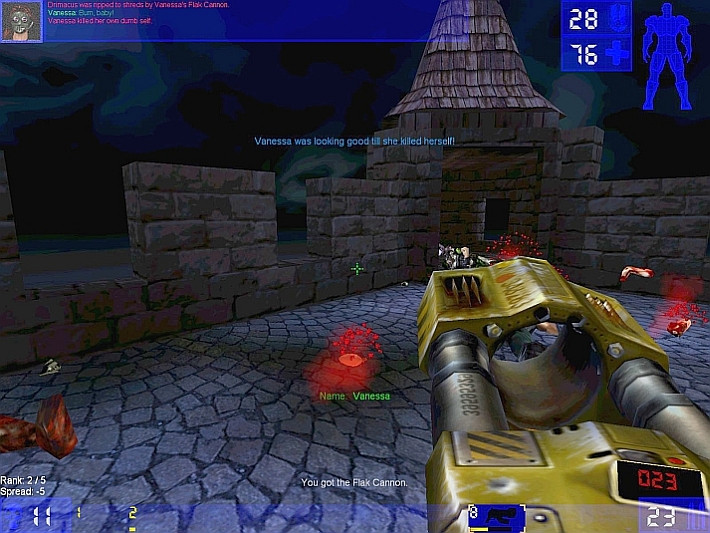
\includegraphics[width=.60\textwidth]{./imagenes/ut.jpg}
\caption{Unreal Tournament}
\label{Unreal Tournament}
\end{center}
\end{figure}
Unreal Tournament \footnote{\url{http://store.steampowered.com/app/13240/}} Unreal Tournament, también conocido como UT y llamado en ocasiones UT99, UT Classic, UT1, o UT:GOTY para diferenciarlo de sus sucesores (Unreal Tournament 2003, Unreal Tournament 2004 y Unreal Tournament 3), es un videojuego de acción en primera persona. 
Lanzado al mercado en 1999, es la continuación del juego Unreal de Epic Games, y su principal enfoque es la acción para multijugador. Compite directamente con el juego Quake III Arena de id Software, que salió al mercado diez días después. Si bien se considera que su competidor tiene mejores gráficos, una buena jugabilidad y un motor gráfico extensamente adoptado, UT tiene una inteligencia artificial superior, una movilidad más variada, y un "disparo alternativo" para las armas, lo que introdujo varios elementos más para la estrategia, más una larga variedad de capacidades multijugador.3

\subsubsection{¿Por qué es uno de mis juegos favoritos?}
\begin{itemize}
\item[Victor Alvarado] La verdad  cuando era pequeño fui a una feria de computacion y vi corriendo castle wolfenstein en una IBM, era lo maximo desde ahi empezo mi gusto por los FPS, siguio los  clasicos como Doom, Doom 2, Heretic, Hexen, Descent , Duke Nukem 3D y unos cuantos mas que son clasicos, pues la competencia empezo.
\end{itemize}
\section{Top Gear}

\begin{figure}[htbp]
\begin{center}
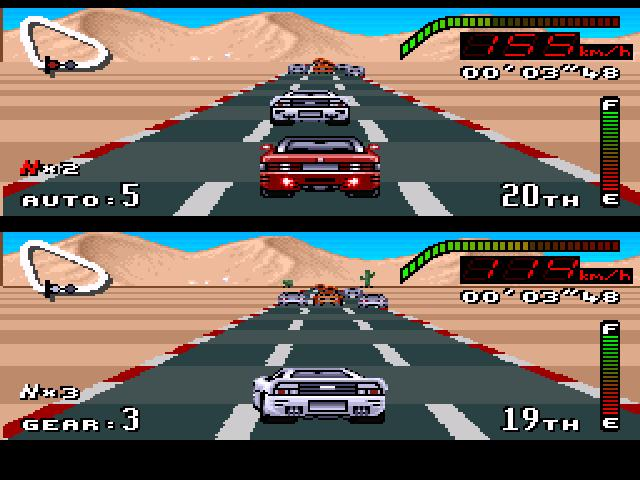
\includegraphics[width=.60\textwidth]{./imagenes/top_gear.jpg}
\caption{Top Gear}
\label{Top Gear}
\end{center}
\end{figure}
Top Gear\footnote{\url{http://es.wikipedia.org/wiki/Top_Gear_(videojuego)}} es un videojuego de carreras para Super Nintendo publicado en el año 1992. En el juego tienes que competir con 20 automóviles para llegar en el primer lugar y avanzar hacia el siguiente torneo. El modo de juego es sencillo, tan solo debes debes indicar mediante teclas la direción a la cual deseas que se dirija el auto.

\subsubsection{¿Por qué es uno de mis juegos favoritos?}
\begin{itemize}
	\item[Saulo Ronquillo]No es un juego muy complejo ni goza de gráficas espectaculares pero hasta el día de hoy me sigue entreteniendo mucho, durante el transcurso del juego las competencias se realizan en diferentes lugares del mundo lo cual ayuda a que el juego no sea monótomo y agregado a todo eso, la música\footnote{\url{http://archive.org/details/TopGearMusicaSnes}} del videojuego es muy, muy buena.
\end{itemize}

\section{Othello (Reversi)}

\begin{figure}[htbp]
\begin{center}
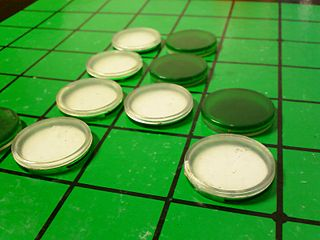
\includegraphics[width=.60\textwidth]{./imagenes/othello.jpg}
\caption{Othello}
\label{Othello}
\end{center}
\end{figure}
El reversi, Othello o Yang \footnote{\url{http://es.wikipedia.org/wiki/Othello}} es un juego entre dos personas, que comparten 64 fichas iguales, de caras distintas, que se van colocando por turnos en un tablero dividido en 64 escaques. Las caras de las fichas se distinguen por su color y cada jugador tiene asignado uno de esos colores, ganando quien tenga más fichas sobre el tablero al finalizar la partida. Se clasifica como juego de tablero, abstracto y territorial; al igual que el go y las amazonas.

La movilidad media de un jugador a lo largo de la partida es de 8 movimientos. Como en total se pueden hacer 60 movimientos, el número máximo de posibles partidas es de aproximadamente $10^{54}$. Por otra parte, el número máximo de posiciones posibles se calcula aproximadamente en $10^{30}$.

\emph{http://es.wikipedia.org/wiki/Othello 2013-05-18}

\subsubsection{¿Por qué es uno de mis juegos favoritos?}
\begin{itemize}
	\item Porque aun cuando parece un juego simple, tiene mucha profundidad. Es muy fácil de aprender, en razón de que las reglas son pocos y sencillas. Además hay versiones por todas plataformas.
\end{itemize}

\section{Sonic Generations}

Sonic Generations\footnote{\url{hwww.sega.com/sonicgenerations/‎} es un juego multiplataforma el cual ofrece una nueva experiencia en juego debido a que sus niveles son llevados a escenarios 2D y 3D recreando el ambiente del Sonic antiguo y del nuevo Sonic respectivamente. Este juego salió para PS3, Xbox360 y PC.
\section{Arcane Legends}

\begin{figure}[htbp]
\begin{center}
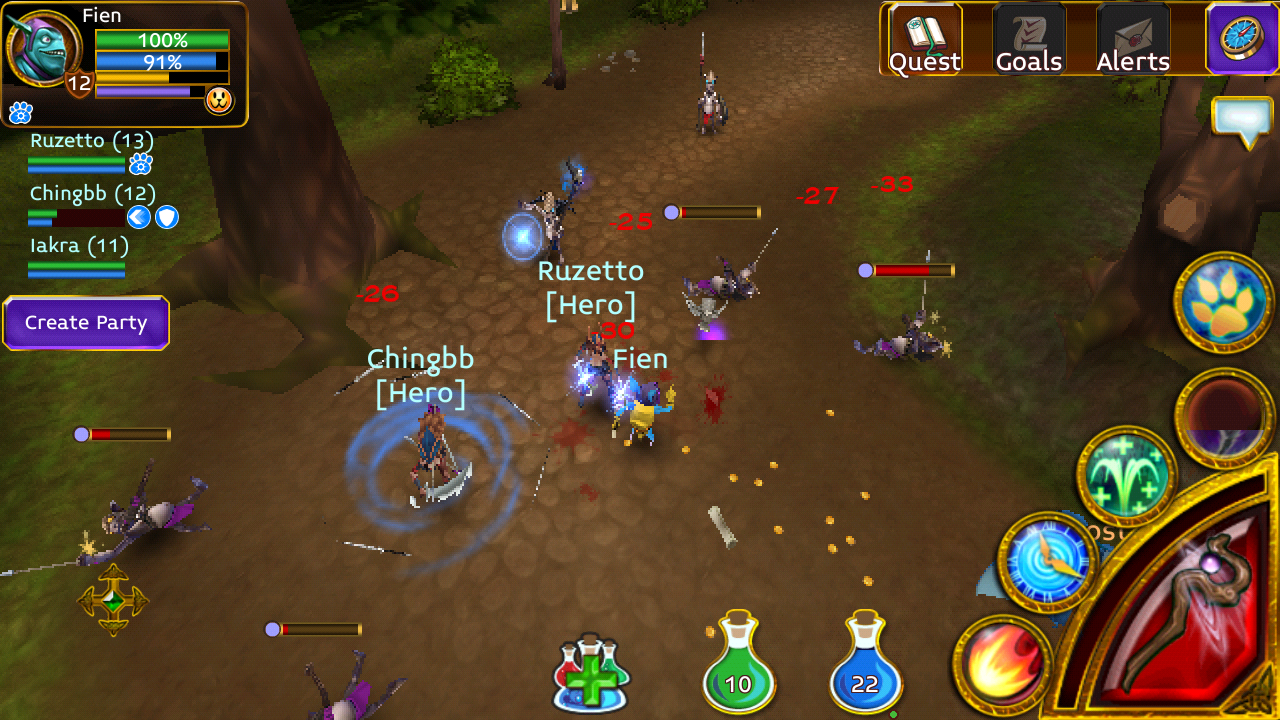
\includegraphics[width=.60\textwidth]{./imagenes/arcanelegends.png}
\caption{Arcane Legends}
\label{Arcane Legends}
\end{center}
\end{figure}
Arcane Legends\footnote{\url{http://www.arcanelegendsgame.com/}} es un juego para plataformas móviles de tipo MMORPG totalmente gratuito en el que podrás combatir en modo cooperativo con otros usuarios de la red y derrotar el mal que encontrarás por todas partes. El personaje que elijas marcará tu personalidad y puedes elegir tres tipos: un pícaro, un mago o un guerrero. Una de las mejores características del juego se basa en un compañero animal que llevas a tu lado y que podrás mandar a tu antojo para que te ayude en la lucha. Además podrás hacerle evolucionar y añadirle poderes extra.

\subsubsection{¿Por qué es uno de mis juegos favoritos?}
\begin{itemize}
\item[César Madrid]Arcane Legends en un juego que te ayuda a entretenerte en tus tiempos libres jugando con conocidos o descocidos a través de la red, en el cual puedes formar grupos para ir avanzando por nuevos mapas o puedes unirte a batallas de jugador contra jugador donde puedes ir demostrando tus habilidades con tu personaje y tu trabajo en equipo con el resto de tu grupo para así poder conseguir la victoria. Lo mejor de este juego es que aparte de jugarlo en tu pc a través de un navegador, también puedes jugarlo desde dispositivos móviles, como android e iOS, y así poder entretenerte en cualquier momento.
\end{itemize}

\section{Crysis 2}

\begin{figure}[htbp]
\begin{center}
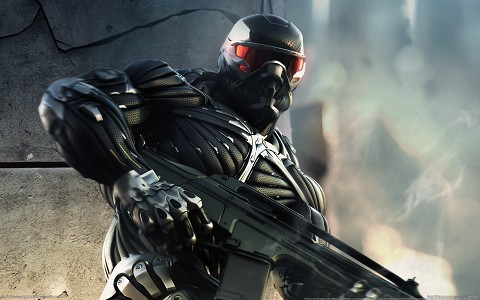
\includegraphics[width=.60\textwidth]{./imagenes/crysis2.jpg}
\caption{Crysis 2}
\label{Crysis 2}
\end{center}
\end{figure}
Crysis 2 \footnote{\url{http://www.ea.com/es/crysis2}} es un videojuego de disparos en primera persona desarrollado por la empresa Crytek y distribuido por Electronic Arts. Fue publicado en marzo del 2011 para PC, Xbox 360 y PlayStation 3. Es la secuela de Crysis y el primer videojuego en usar el motor CryEngine 3 desarrollado por Crytek también.

\subsubsection{¿Por qué es uno de mis juegos favoritos?}
\begin{itemize}
\item[Rubén Carvajal] La esencia del juego es magnífica, la historia consigue atraparte con su argumento futurístico.
Uno puede jugarlo a su manera, dependiendo del escenario habrán momentos en que te guste más pasar a todos descargando todo tu arsenal de armas, o momentos en que lo que sirva más sea utilizar las múltiples opciones del traje y el sigilo.
La jugabilidad y los gráficos son de altísima calidad, las opciones de camuflaje y el entorno en el que se desarrolla el juego son particularidades destacables.

El sonido de cada ambiente está bien trabajado, e incluso tenemos opciones gráficas en 3D, cosas que hacen de este un excelente juego.
\end{itemize}

\section{Super Smash Bros. Melee}

\begin{figure}[htbp]
\begin{center}
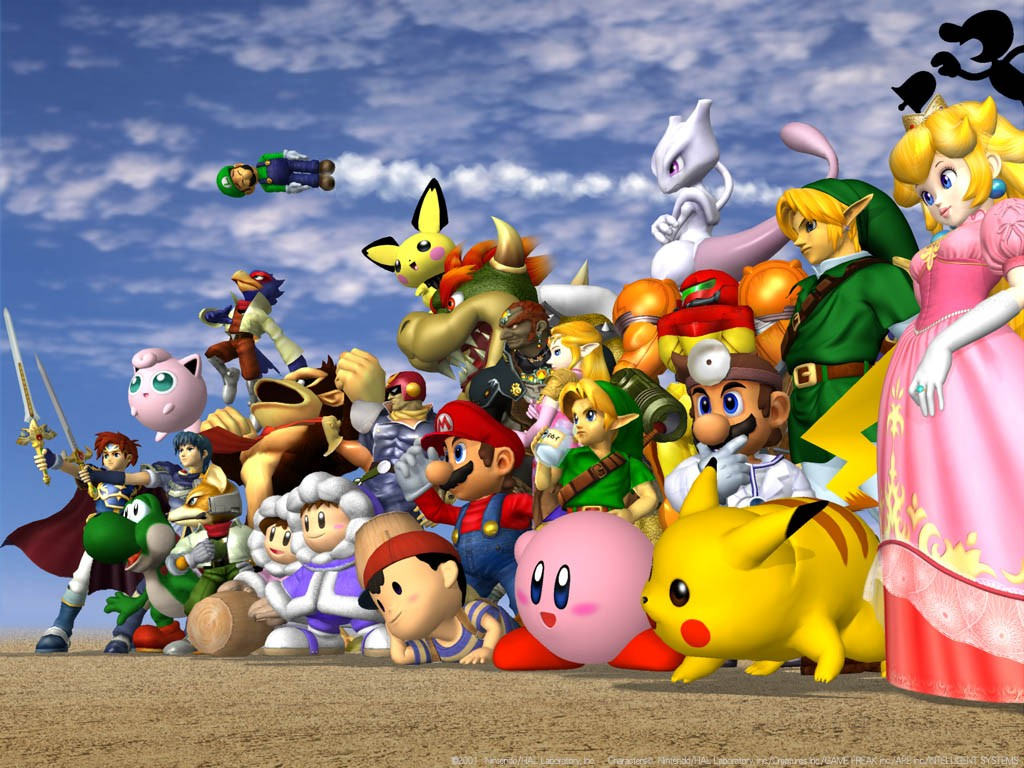
\includegraphics[width=.50\textwidth]{./imagenes/SuperSmashBrosMelee.jpg}
\caption{Super Smash Bros. Melee}
\label{Super Smash Bros. Melee}
\end{center}
\end{figure}
Super Smash Bros. Melee trata de un juego de lucha en dos dimensiones con gráficos en 3D protagonizado por 26 estrellas de Nintendo (Figura \ref{Super Smash Bros. Melee} ) de todos los tiempos. Se trata del juego más vendido de GameCube, con unas ventas superiores a 6 millones de copias en todo el mundo.

\subsubsection{¿Por qué es uno de mis juegos favoritos?}
\begin{itemize}
\item[Danny Ponce] Super Smash Bros. Melee es demasiado entretenido por su variedad en el modo de juego para un solo jugador que son cuatro: Regular Match, Event Match, Stadium, Training y para multijugador son tres: Melee, Tournament Melee y Special Melee. Este juego se deben desbloquear 11 estrellas del Nintendo, Escenarios y Trofeos jugando en cualquiera de los modos. Para mi, El modo más entretenido es Melee que puede jugar hasta 4 personas. Si hay menos de Cuatro personas para jugar, se puede seleccionar luchadores controlados por la CPU en niveles de dificultad del 1 al 9. Se pueden configurar las reglas del juego para luchar en equipos o individual y luchas por tiempo o con un número de vidas prefijado, con diferentes condiciones de victoria, como un sistema de monedas por el que con cada golpe un luchador suelta monedas y gana quien más recoge. También se puede escoger la frecuencia con la que aparecerán ítems en el escenario, desactivar algunos o todos.Una vez listos los jugadores, aparece la pantalla de selección de escenario, pudiendo elegirlo manualmente entre los desbloqueados o permitir a la consola seleccionarlo aleatoriamente.
\end{itemize}
\section{Counter-Strike}

\begin{figure}[htbp]
\begin{center}
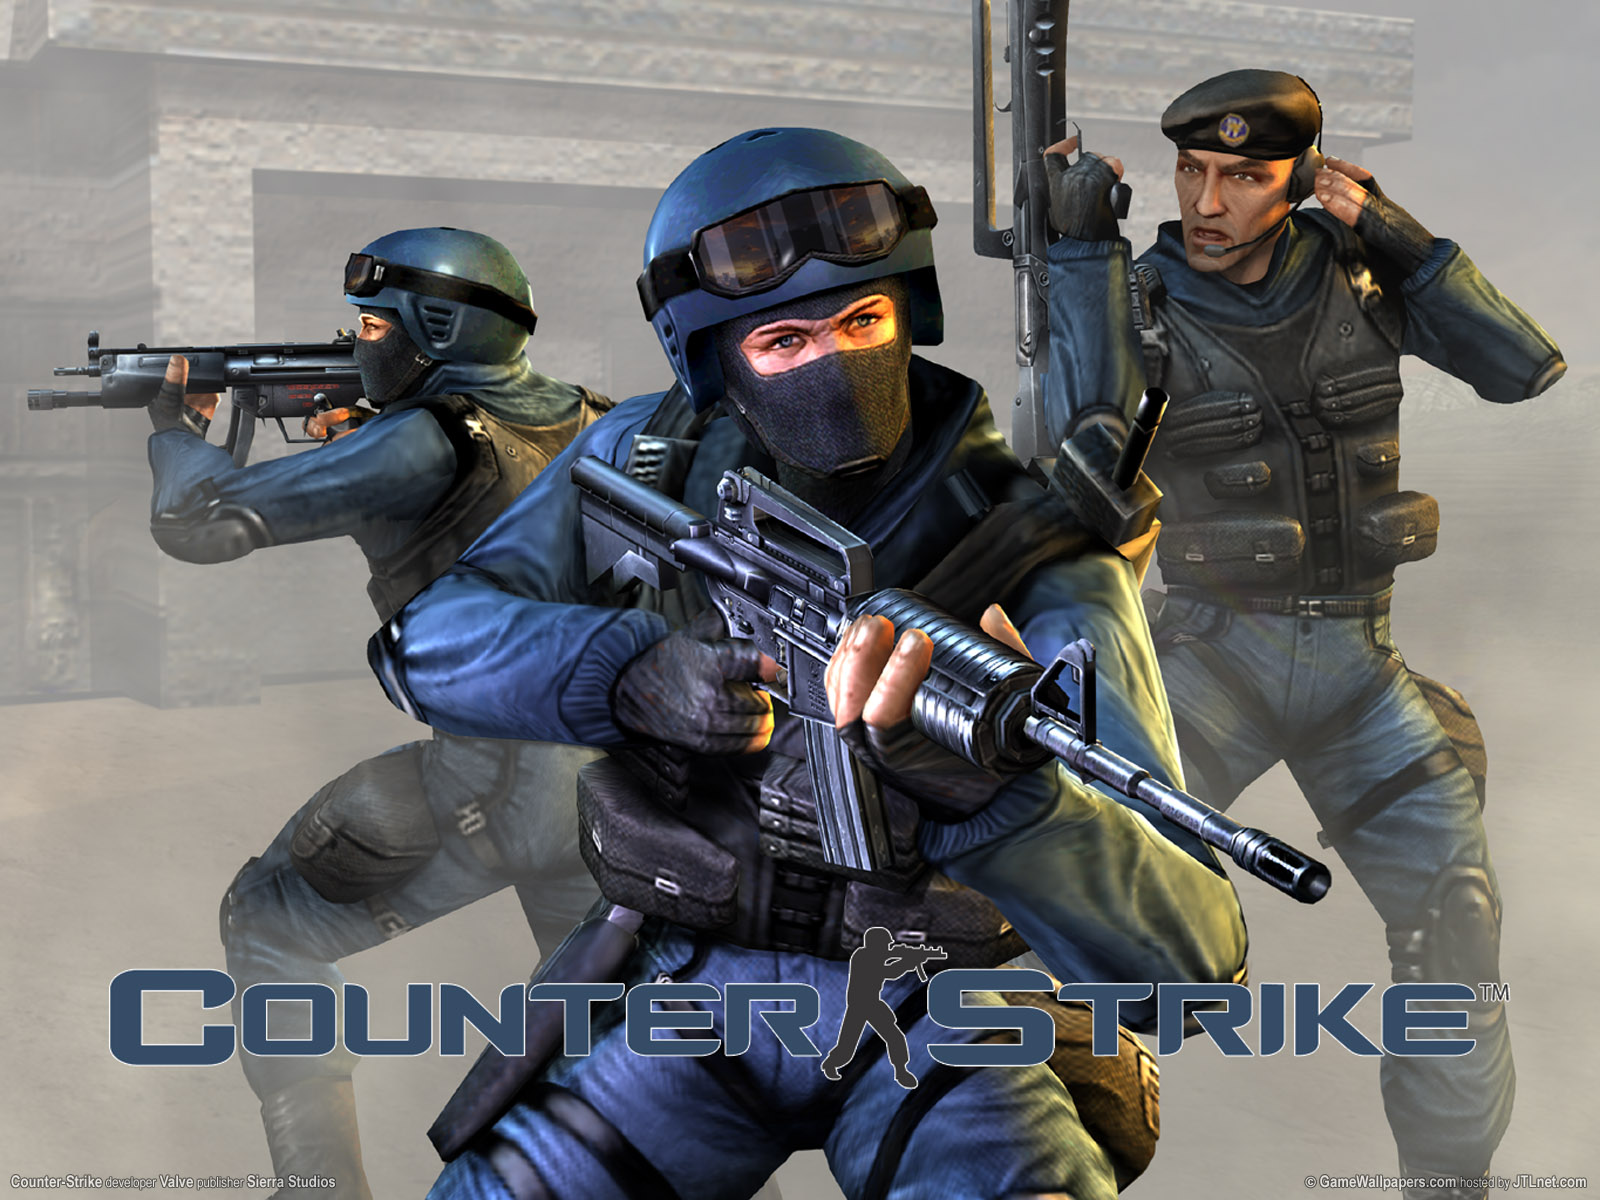
\includegraphics[width=.60\textwidth]{./imagenes/CounterStrike.jpg}
\caption{Counter-Strike}
\label{Counter-Strike}
\end{center}
\end{figure}
Counter-Strike\footnote{\url{http://http://store.steampowered.com/css/}} es un juego de tipo multijugador. La acción de Counter-Strike se desarrolla en rondas de una duración elegida por el que las crea, en la cual un equipo de terroristas se enfrenta a un equipo de antiterrorista. El equipo victorioso es el que cumpla todos sus objetivos de victoria, de situación o la eliminación de todos los jugadores del otro equipo. Si al final de la ronda no hay victoria directa de uno de los dos equipos, el equipo que no realizó sus objetivos pierde por eliminación.

\subsubsection{¿Por qué es uno de mis juegos favoritos?}
\begin{itemize}
\item[Edwin Hermenejildo] Counter-Strike Agrupa varios aspectos del espíritu deportista: trabajo de equipo, competencia, igualdad de oportunidades y con su éxito es lógico que el juego haya dado a un gran número de jugadores el deseo de competir.
Todos los jugadores comienzan con la misma cantidad de puntos de vida y la cantidad de puntos de armadura que consiguieron conservar durante la ronda anterior siempre y cuando no compren una nueva. Cuando los daños son causados por los disparos de sus adversarios o sus compañeros -si hay fuego amigo- (los compañeros causan menos daño, pero pueden matar igualmente), así como por una caída violenta los puntos de vida del jugador disminuyen. Los disparos se pueden localizar en diferentes partes del cuerpo (brazo derecho e izquierdo, pierna derecha e izquierda, torso, y cabeza), y causan más o menos daños según el lugar afectado, sabiendo que un disparo en la cabeza o headshot es a menudo mortal. La pérdida de puntos de vida solo causa una pequeña disminución en los movimientos del terrorista o antiterrorista que haya recibido el daño. Cuando la totalidad de los puntos de vida se terminan, el jugador muere.
\end{itemize}

\section{God Of War III}

\begin{figure}[htbp]
\begin{center}
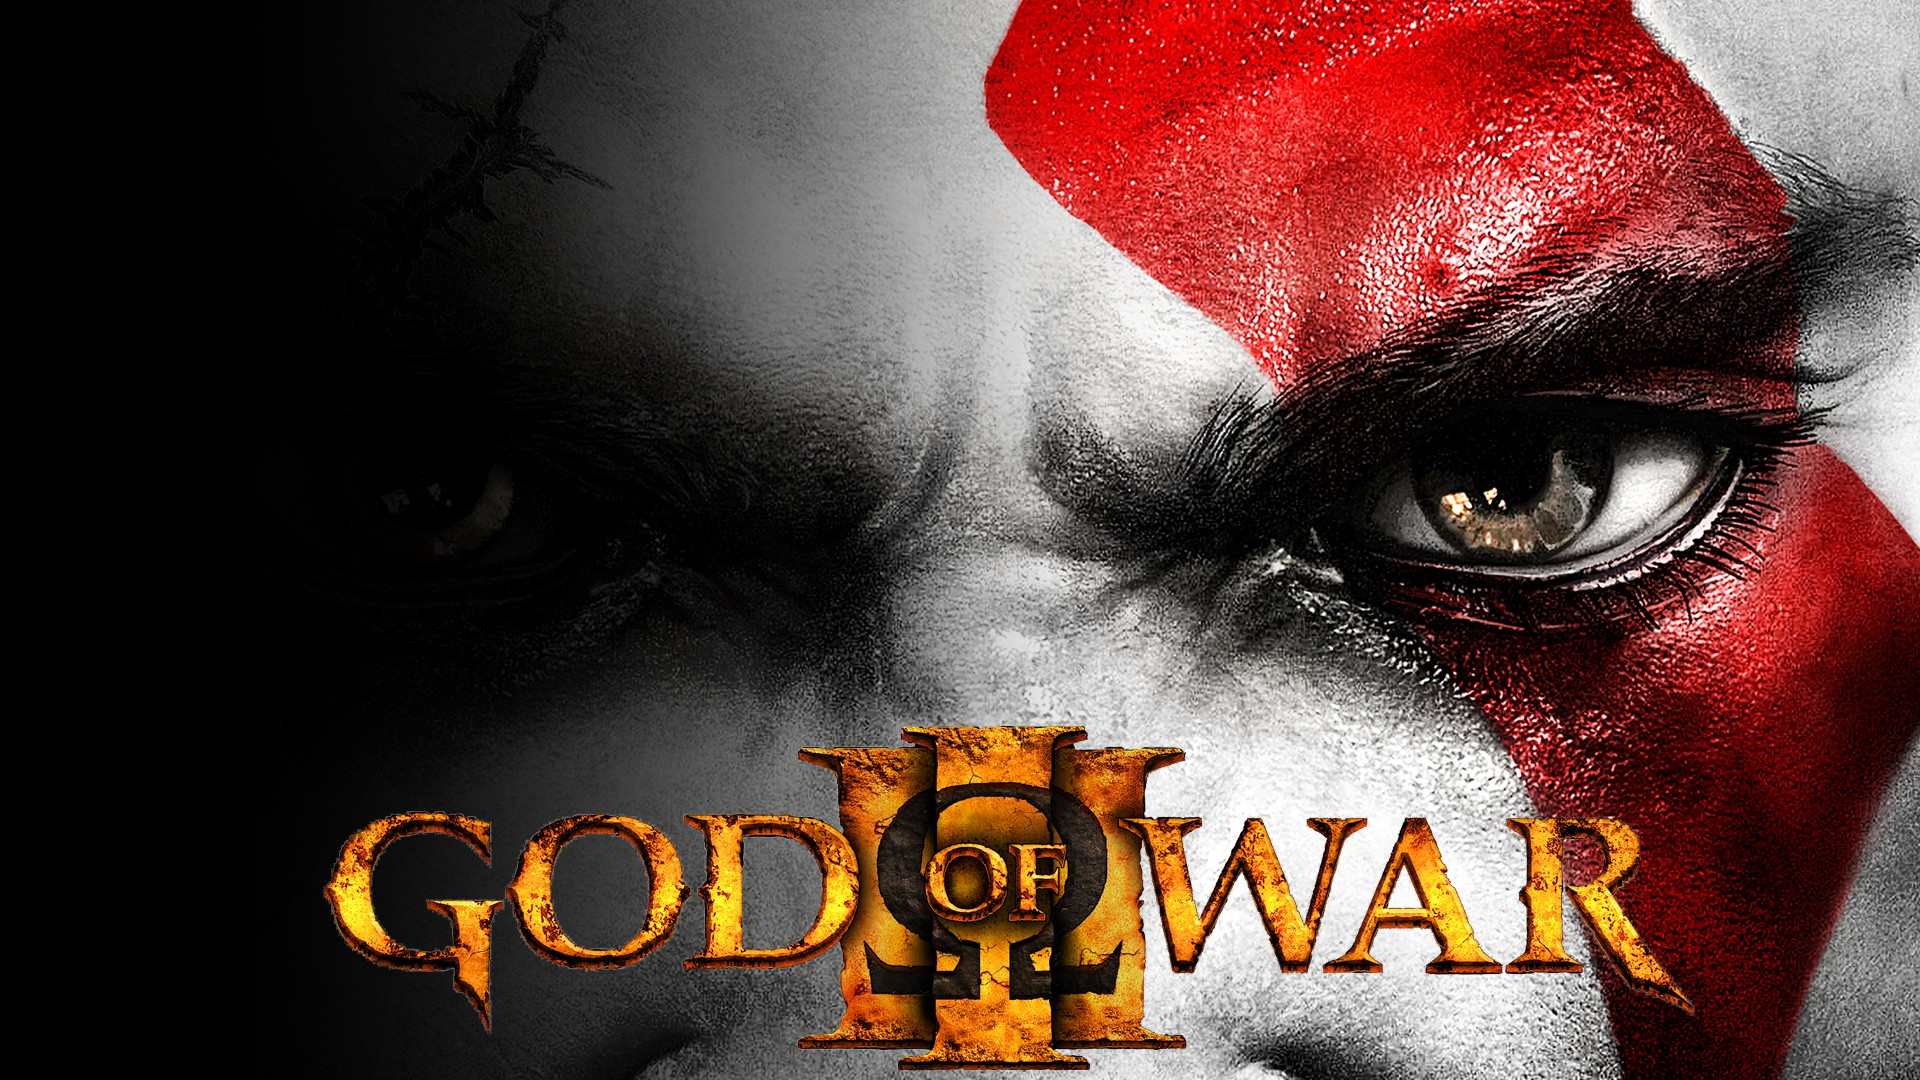
\includegraphics[width=.60\textwidth]{./imagenes/godofwar3.jpg}
\caption{God Of War III}
\label{God Of War III}
\end{center}
\end{figure}
God Of War III\footnote{\url{http://www.ign.com/games/god-of-war-iii/ps3-886158/}} God of War III es un juego basado en la mitologia griega, en donde el personaje principal llamado Kratos, el cual era el antiguo Dios de la Guerra, asciende al olimpo con la ayuda de los Titanes para tomar venganza de Zeus ya que éste lo habia traicionado. Ya en el olimipo se enfrentara a todos los dioses que habitan ahi, incluidos los tres mas poderosos Hades, Poseidon y por ultimo Zeus, pero Kratos estara ayudado por Atenea quien lo guiará a lo largo del juego y le dara la clave para poder derrotar a Zeus. 

\subsubsection{¿Por qué es uno de mis juegos favoritos?}
\begin{itemize}
\item[Kevin Silva] El juego es muy real, ha sido premiado por la calidad de graficos y su trama es muy envolvente. Tambien posee minijuegos de logica a lo largo que vas avanzando por el juego. El juego no es muy corto pero tampoco muy extenso y en el camino podras encontrarte con muchos enemigos, tambien poder controlar un sinnumero de armas conforme vayas ganado batallas y a la vez escoger cual de ellas aumentarles de poder. En fin el juego te da muchas posibilidades y brinda garantia de que no te aburrirás al jugarlos, es por ésta razon que fue catalogado como el "Videojuego mas esperado del 2010"  
\end{itemize}

\section{Sims}

\begin{figure}[htbp]
\begin{center}

\includegraphics[width=.60\textwidth]{./imagenes/Logo_of_The_Sims_(2013).png}
\caption{Sims}
\label{Sims}
\end{center}
\end{figure}
Sims\footnote{\url{http://www.thesims3.com/}} es un juego de computadorra que salio el 2000 por parte de Electronic Arts. El juego en si es un simulador estrategico de vida, en el cual el jugador crea gente virtual llamados "Sims" y los ayuda a desarrollar su vida y satisfacer sus necesidades. Estos pueden vivir en casas pre-fabricadas o el jugador puede construirlas por si mismos.

\subsubsection{¿Por qué es uno de mis juegos favoritos?}
\begin{itemize}
\item[Alvaro Ortiz] El juego en si se presenta con la metodologia de "Sandbox" la cual no presneta ninguna meta aparte de que tus Sims sobrevivan dando rienda suelta a lo que el jugador puede lograr con el juego. En si todo se vale, puedes crear una familia, llegar a una alta profesion, convertirte en cosas raras, e incluso matar tu personaje y el juego no te limita de ninguna manera. Otro aspecto que me parece atrayente es en la creacion de casas y edificios el cual permite usar una larga gama de objetos y tecnicas para construir los disenios mas exhuberantes que una pueda concebir mediante la creatividad del usuario. Incluso si te aburres cada cierta cantidad de tiempo siguen saliendo expansiones para aumentar las posibilidades de desarrollo de la "historia" del juego con grandes cantidades de contenido nuevo.
\end{itemize}
\section{Mario Kart 64}

\begin{figure}[htbp]
\begin{center}
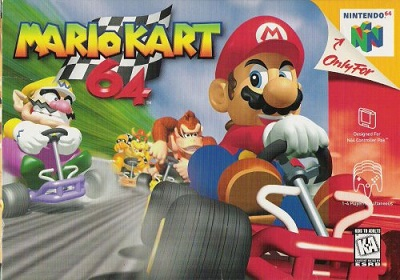
\includegraphics[width=.60\textwidth]{./imagenes/kart1.jpg} 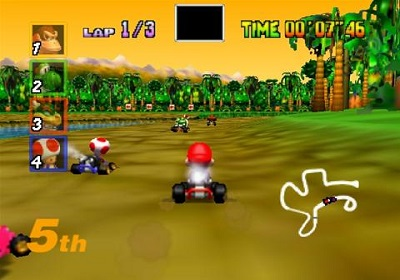
\includegraphics[width=.60\textwidth]{./imagenes/kart2.jpg} 
\caption{MarioKart}
\label{Mario Kart}
\end{center}
\end{figure}

\begin{itemize}
\item[Dennise Pintado] Ahora en un mundo donde el poder computacional de las maquinas hacen que todos deseemos  gráficos cada vez más realistas, nos encontramos con gustos algo antiguos u obsoletos pero a mi parecer es como las películas o músicas clásicas, nunca pasaran de moda. Cuando mis padres compraron la consola del Nintendo 64 el primer juego a probar fue el MarioKart 64,  con  64 bits de potencia gráfica la inmersión producida en el juego  por estos gráficos 3D llenos de colores, combinado con la iluminación de las carreteras en las que se corría, los efectos de sonido de cada estrella, cascaron, bananas  y el vibrar del control de mando cuando topaba con alguna de estas, me hacían sentir una experiencia de usuario fantástica. Con sus cuatro entradas se podían disfrutar de experiencias multijugador y el  control del juego que se tenía con este  mando era único, ya que su diseño era totalmente adaptable a la mano y daba un control de 360 grados alrededor de la escena que se jugaba.  
\end{itemize}

\section{guitarHERO2}

\begin{figure}[htbp]
\begin{center}
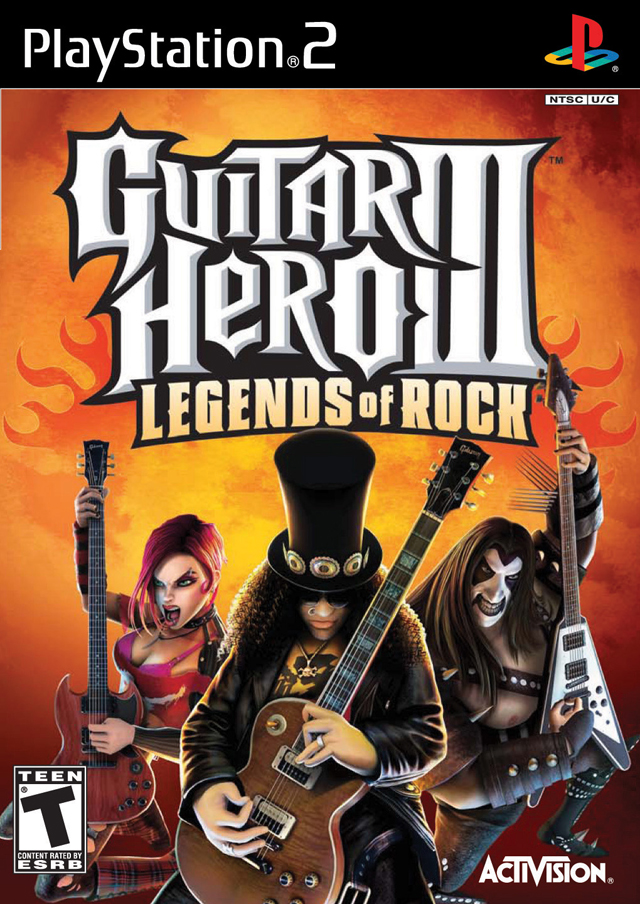
\includegraphics[width=.60\textwidth]{./imagenes/guitar.jpg} 
\caption{Guitar Hero 2 Playstation 2}
\label{Guitar Hero2}
\end{center}
\end{figure}


\begin{itemize}
\item[Keyla Figueroa] Por qué este juego? Me gusta el juego porque es muy entretenido a pesar de no ser rockera con este juego logré conocer más acerca de los mejores guitarristas de este género, disfruto mucho de todas las canciones y pienso que practicarlo continuamente podría estimular la movilidad en las manos.
\end{itemize}

\chapter{Conclusiones}
Cuales juegos fueron más populares y un breve razonamiento del porqué.

\end{document}  
